\section{Yorkshire}
\begin{marginfigure}
\begin{tikzpicture}
\node [name-dest] (box){%
    \begin{minipage}{0.80\textwidth}
     \begin{itemize}
    \item Oliver Myerscough
    \item Jack Hare
    \end{itemize}
    \end{minipage}

};
\node[fancytitle, right=10pt] at (box.north west) {Slinging in the Rain};
\end{tikzpicture}
\end{marginfigure}

I’d missed expo in my first year, and deeply regretted it. After two years of hearing breathless tales of caverns measureless to man, listening to Black Adder in a camp buried in 600 m of rock and shitting in a small plastic bag, I couldn’t be more excited to go underground. And who could be a more suitable and enthusiastic caver to go with than Oli? I’d had a busy day - pushing M10 at 6 am (Surely the log book lies?) with Rhys, killed it by 9 am, a walk up Kuk and some surface bashing, back to cook dinner and then heading off for UG with Oli at 7 pm.

We were going to set up camp, so we had a few bags with us and more to collect along the way. The previous bounce trip I’d done with Rhys we’d left Zimmer unrigged, confidentally assuming that neither of us would be involved in the next trip. Oli swung around in the darkness looking for spits and grumbling, but soon we were down, bags of comf and electronics swinging from my hips, into the drippy, bouldery chamber of Zimmer.

\begin{marginfigure}
\checkoddpage \ifoddpage \forcerectofloat \else \forceversofloat \fi
\centering
 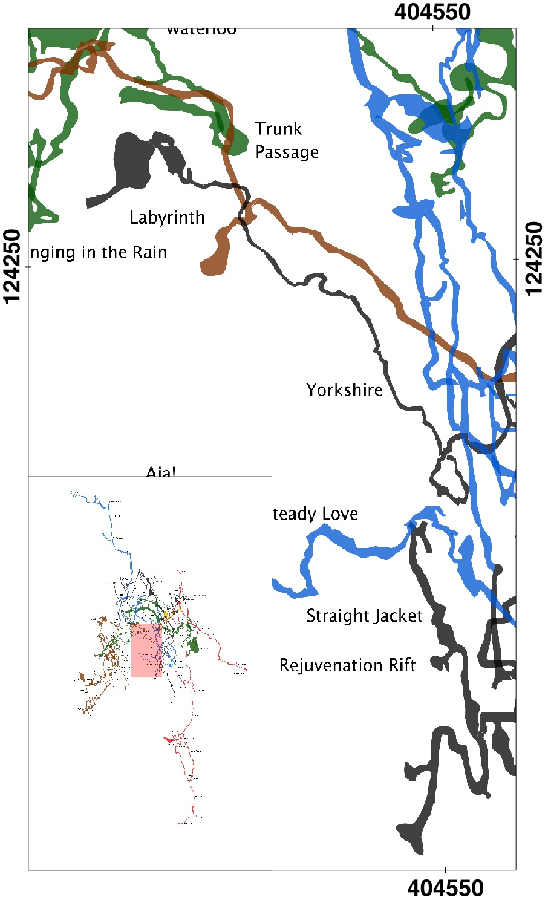
\includegraphics[width=\linewidth]{2015/jack-yorkshire-2015/labyrinth_inset}
 \caption{Plan view of the \emph{Yorkshire extensions}, Slovenian National Grid ESPG 3794}
 \label{Labyrinth inset}
\end{marginfigure}

Oli had gone ahead so I had no idea where to go from here, but he soon came back and showed me the way, pointing out the sights of Camp X-ray along the way. We got the camp set up, sorted out the rotten food from the good, unpacked the comf and lit some candles. Not as much work as I’d been lead to believe, but Camp X-ray is a work of art and very well made. Quite soon I was asleep, and I have never slept more deeply or more deeply.



I awoke with a start 10.5 hours later. Oli showed me how to make tea without getting out of the sleeping bag, and after an obligatory shit we were off, down a muddy slope from Friendship Gallery and into Yorkshire. I don’t remember much of the route, classic fresher trying so hard to keep up that I didn’t note any landmarks. I recall a grim vertical crawl into a winding rift that had apparently been dug, which then widened to the Yorkshire-eqsue qualities I’d been promised.

Soon we were at the pushing front, a pitch that Oli had found two years before and wanted to bolt. Looking at it, I decided it was very free climbable, only 5 m tall and with wide ledges flaring out from the wall of the old streamway. Oli concurred and we were quickly down, greeted by a window into a chamber. A quick flash of the light showed the deviation sling for Slinging In the Rain, so we had killed this lead. 

A bit disgruntled, we decided to go back up and round to check out the boulder at the end of Slinging in the Rain. Down the slightly wet pitch, and round the streamway into the little oxbow. Well, that was a rock alright, quite large and filling the passage. I couldn’t see much passed it - at the time I thought it didn’t look hopeful, but I have seen worse since that have gone. Oli and I wrapped a sling around it and tried all the tricks we’d learned in NZ for getting the boulder out, but we couldn’t shift it. It needs bang or plugs and feathers.

We climbed back out and found a neat chamber off the side of the main passage. It had clearly had a swirling plunge pool at the bottom, but what was neat was that half way up it had cut through an upward sloping phreatic passage. Oli backtracked and found a way into the phreatic. Lying there on his back he attempted to put a bolt in so we could try and climb higher into another phreatic entering at the top of the chamber. He quickly gave up, as the position was awkward. I attempted to hook some slings over spikes and get higher by progressively doing this, but it was a bit hopeless and we gave up after about an hour.

\begin{figure*}[t!]
\checkoddpage \ifoddpage \forcerectofloat \else \forceversofloat \fi
\centering
\frame{\includegraphics[width=\textwidth]{"2015/jack-yorkshire-2015/Jack-Area-N (1)".jpg}}
\caption{The jagged limestone peaks of the Krn massif provide the perfect backdrop for a day of hiking near Kuk --- In the foreground Jack Hare negotiates the tricky mountain path --- Rhys Tyers}
\label{kukjack}
\end{figure*}

On the way back a side passage proved to be a long way to get back to the main passage, but it was at least entertaining. I suspect we didn’t survey it, sorry.

Back at camp, a long sleep and then out. This was my only camping trip in 2015, as the lack of people to go with drove me towards digging Coincidence Cave, but I vowed to be back in 2016 for longer.

\name{Jack Hare}
